% !TeX root = ../main.tex

\section{Resultate}

\begin{frame}{Resultate {\scriptsize \cite[S.~101-102]{stenningHumanReasoningCognitive2008}}}
    \begin{itemize}
        \item jede Manipulation bringt (unterschiedlich gute) Verbesserung
        \item entsprechend Vorhersagen der Theorien, von denen Manipulationen abgeleitet wurden
        \item starke Evidenz für Zusammenhang zwischen Manipulationen und mentalen Vorgängen, auf die sie einwirken
    \end{itemize}
\end{frame}


\begin{frame}{Resultate {\scriptsize \cite[S.~101]{stenningHumanReasoningCognitive2008}}}
    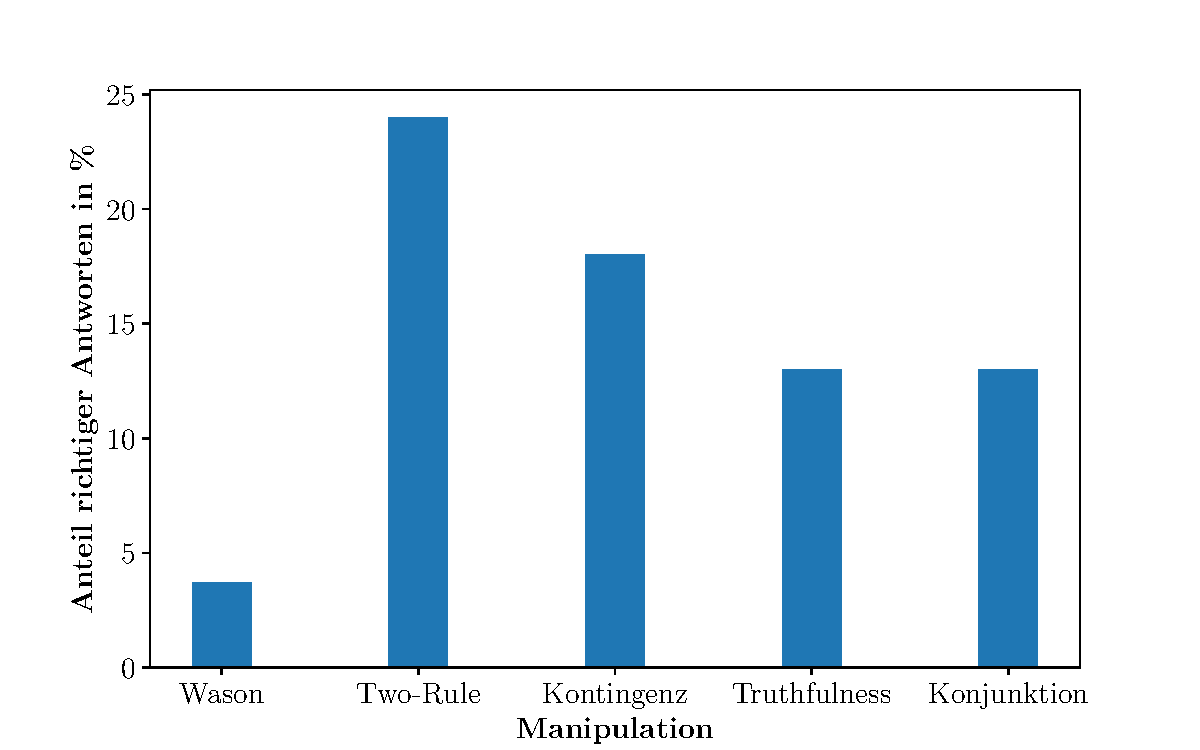
\includegraphics[width=\textwidth]{../plot/results_correct.pdf}
\end{frame}


\begin{frame}{Two-Rule Task {\scriptsize \cite[S.~109]{stenningHumanReasoningCognitive2008}}}
    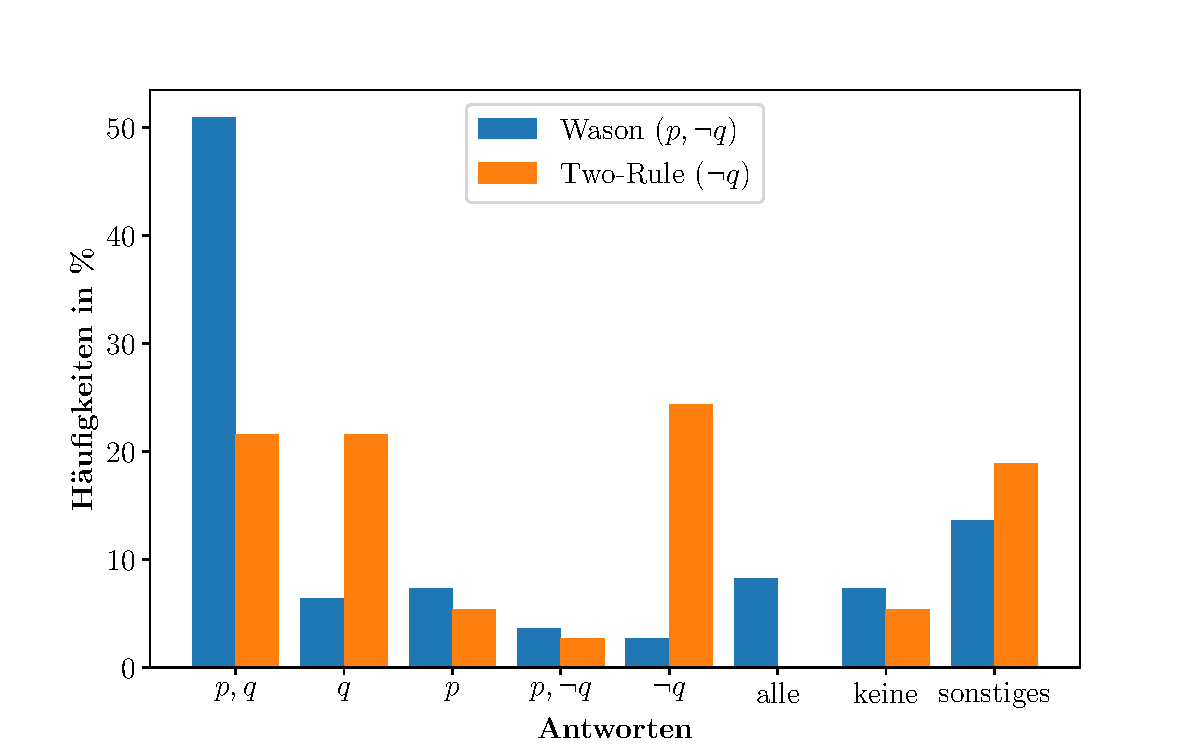
\includegraphics[width=\textwidth]{../plot/results_two_rule.pdf}
\end{frame}


\begin{frame}{Two-Rule Task {\scriptsize \cite[S.~102-104]{stenningHumanReasoningCognitive2008}}}
    $(p \to q) \leadsto (\{U, I\} \to 8)$

    \begin{itemize}
        \item Verwechslungsgefahr zwischen
        \begin{itemize}
            \item \enquote{diese Regel trifft auf diese Karte zu}
            \item \enquote{diese Karte macht diese Regel wahr}
        \end{itemize}
        
        \item $q~\hat=~8$ könnte beide Regeln bestätigen \\
            $\Rightarrow$ Konflikt: eine Regel wahr, eine falsch
        
        \item asymmetrische Beziehung von \emph{true}
        
        \item Information-Gain: $\lnot q$ bietet am meisten Informationen \\
            $\Rightarrow$ Vorhersage: häufigste Wahl
        \begin{itemize}
            % Achtung: hier Widerspruch!
            % Buch schreibt "false-consequent card comes in third"
            % Daten in Tabelle 4.2 und 4.4
            \item Beobachtung: tatsächlich häufigste Antwort
        \end{itemize}
    \end{itemize}
\end{frame}


\begin{frame}{Kontingenz {\scriptsize \cite[S.~109]{stenningHumanReasoningCognitive2008}}}
    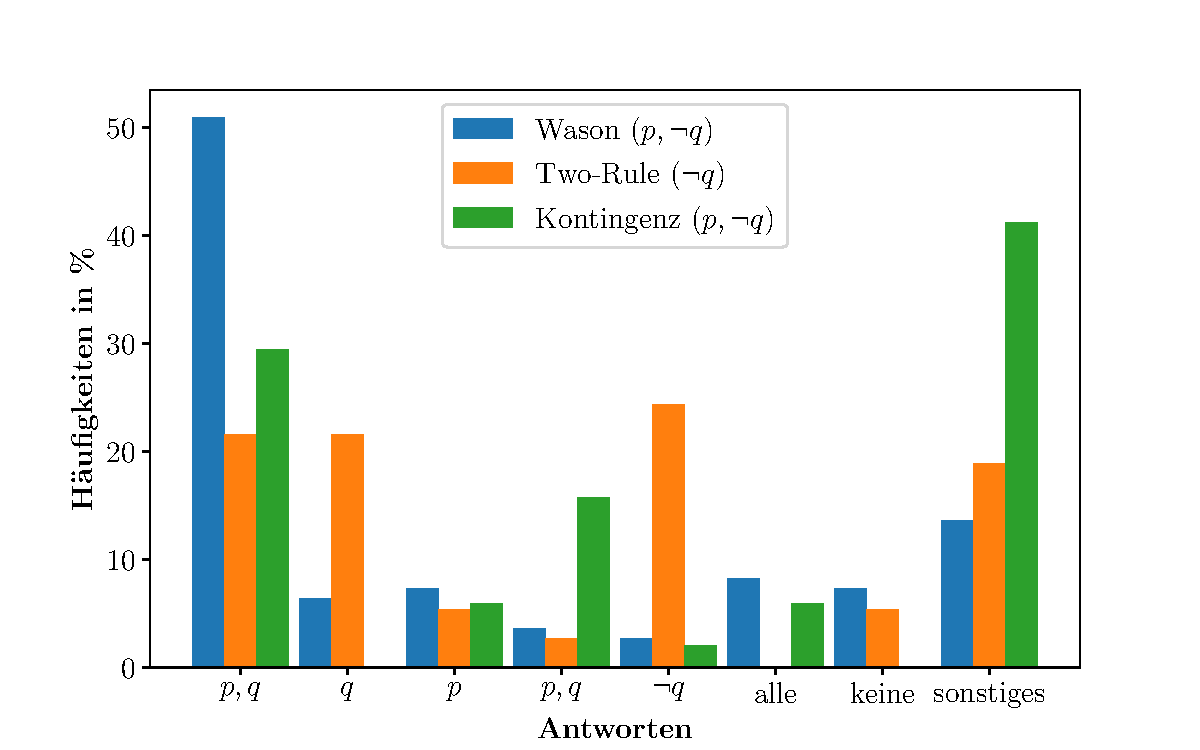
\includegraphics[width=\textwidth]{../plot/results_contingency.pdf}
\end{frame}


\begin{frame}{Kontingenz {\scriptsize \cite[S.~105,109]{stenningHumanReasoningCognitive2008}}}
    Kontingenz $\Rightarrow$ Entscheidung vor weiteren Informationen
    \begin{itemize}
        \item Beobachtung: prognostizierte Wirkung tritt ein {\small (häufiger $\lnot q$)} \\
            $\Rightarrow$ Erklärung für schwerwiegende Unterschiede
        
        \item problematisch für rationale Analysemodell {\small (u.a. Information-Gain)}
        \begin{itemize}
            \item Warum steigt Wahl von $p,~\lnot q$ signifikant? (15,7\% statt 3,6\%)
            \item Einfluss von Kontingenzen der Antworten auf Interpretation schwierig zu erkennen
        \end{itemize}
    \end{itemize}
\end{frame}


\begin{frame}{Interaktive Kontingenz {\scriptsize \cite[S.~105,109]{stenningHumanReasoningCognitive2008}}}
    \begin{itemize}
        \item \textsc{van Denderen}: reaktive Planung als Quelle der Schwierigkeiten
        \item Subjekte dürfen Karten vor Entscheidung drehen (GUI)
        \item Trick: erste Karte falsifiziert nie
        \item Kompetenz-Antwort $(p,~\lnot q)$ nun häufigste Antwort \\
        (26\% statt 3,6\%) \\
        $\Rightarrow$ Verlangen nach reaktiver Planung deutlich problematisch
        
        \item[!] mehrere Veränderungen der Aufgabe
        \item[$\Rightarrow$] Verifikation / Falsifikation
        \item[$\Rightarrow$] Unterschied deskriptiv und deontische Aufgabe:\\
            keine Kontingenzen zwischen Antworten
    \end{itemize}
\end{frame}


\begin{frame}{Truthfulness {\scriptsize \cite[S.~109]{stenningHumanReasoningCognitive2008}}}
    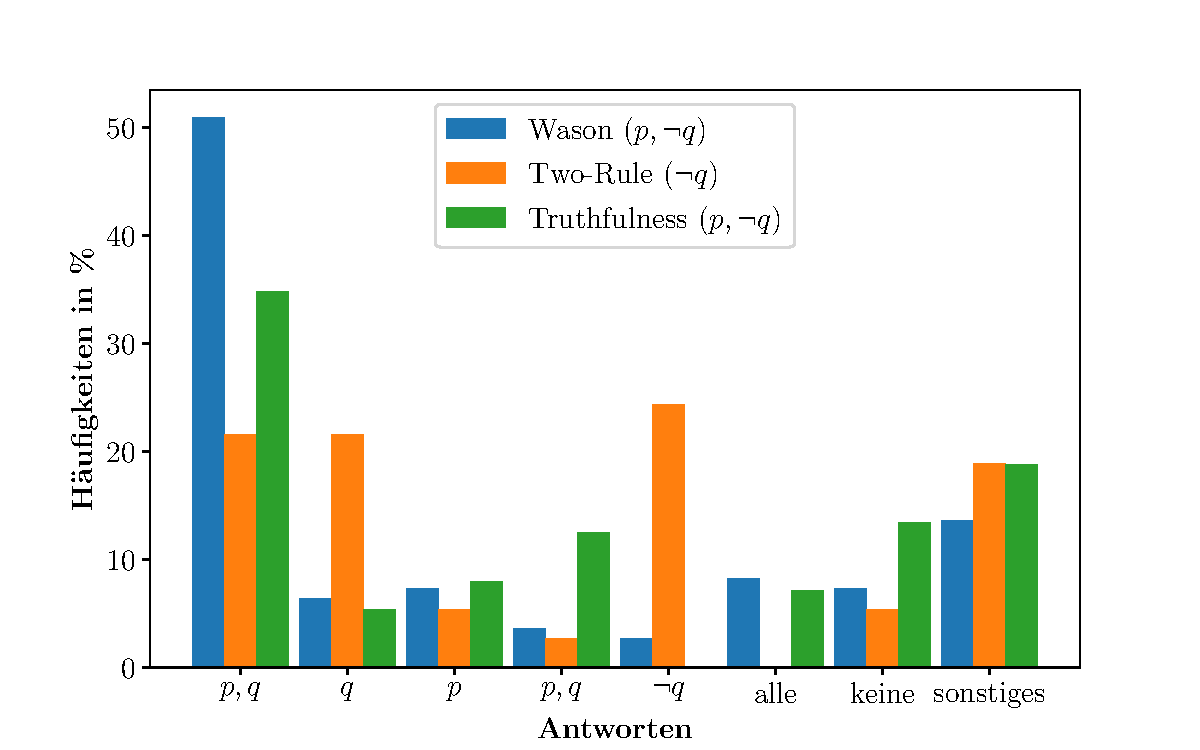
\includegraphics[width=\textwidth]{../plot/results_truthfulness.pdf}
\end{frame}


\begin{frame}{Truthfulness {\scriptsize \cite[S.~107]{stenningHumanReasoningCognitive2008}}}
    \begin{itemize}
        \item Quelle der Regel $\ne$ Experimentator:in
        \item Proband:innen sollen nach Gegenbeispielen suchen
        \item (kleine) signifikante Verbesserung (12,5\% statt 3,6\%)
        \item Ursachen nicht ganz klar
        % TODO: ggf. weiter aufbereiten
    \end{itemize}
\end{frame}


\begin{frame}{Konjunktion {\scriptsize \cite[S.~109]{stenningHumanReasoningCognitive2008}}}
    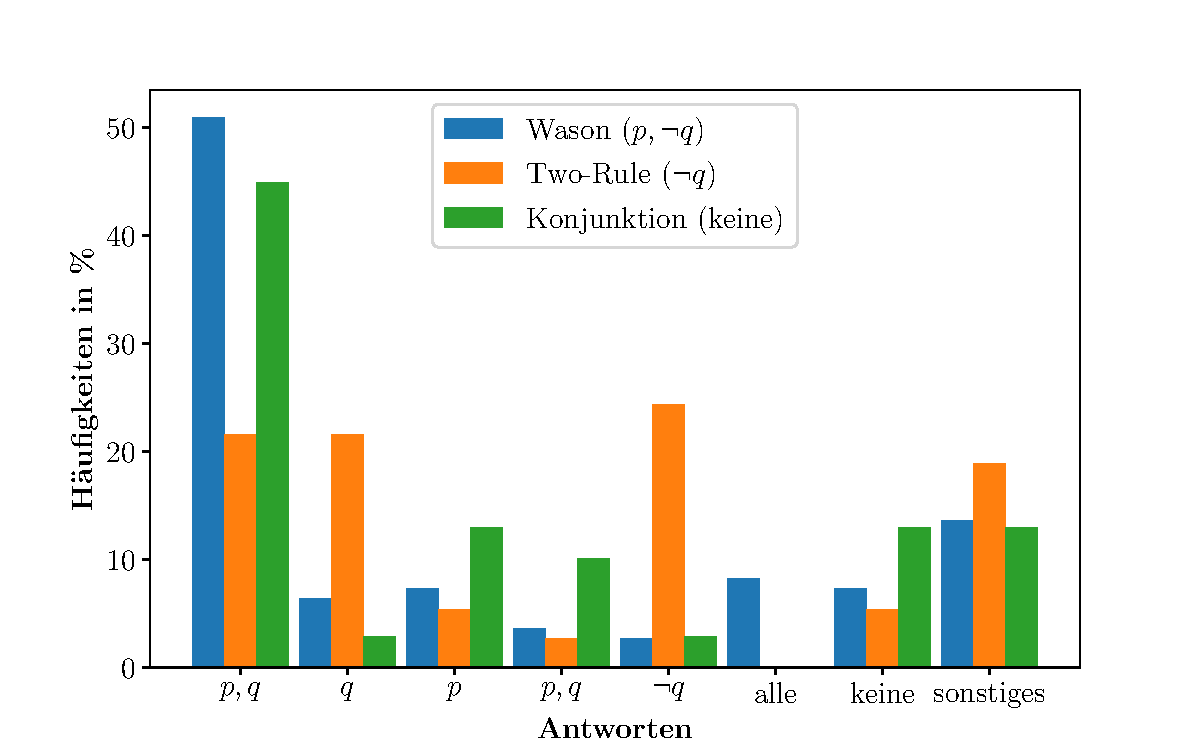
\includegraphics[width=\textwidth]{../plot/results_conjunction.pdf}
\end{frame}


\begin{frame}{Konjunktion {\scriptsize \cite[S.~107-109]{stenningHumanReasoningCognitive2008}}}
    \begin{itemize}
        % \item Intention: Probleme außerhalb von Konditionalen; logische Veränderung
        \item Formbarkeit der Semantik von Sätzen
        \item Beobachtung: Interpretation ähnlich zu \texttt{if ... else ...}
        \item signifikante Steigerung der Kompetenzantwort {\small (13\% statt 3,6\%)}
        % \item häufigste Antwort immer noch ähnlich stark
        
        \item mögliche Ursachen:
        \begin{itemize}
            \item vermehrt deontische Interpretation $\Rightarrow$ Suche nach Verstößen
            \item \textsc{Fillenbaum} zeigt: ca. \sfrac{1}{2} lesen \texttt{if else} {\small (nicht ausreichend)}
            \item Annahme $p$ wahr, entsprechende Folgerung
        \end{itemize}
        
        \item Probleme
        \begin{itemize}
            \item deontisches Lesen indikativer Regeln
            \item Unnatürlichkeit, Satz statt Experimentator:in zu hinterfragen
            \item ähnlich schwere (verschiedene, verwandte) Probleme wie Implikation
        \end{itemize}
    \end{itemize}
\end{frame}


\begin{frame}{Konjunktivisch {\scriptsize \cite[S.~109]{stenningHumanReasoningCognitive2008}}}
    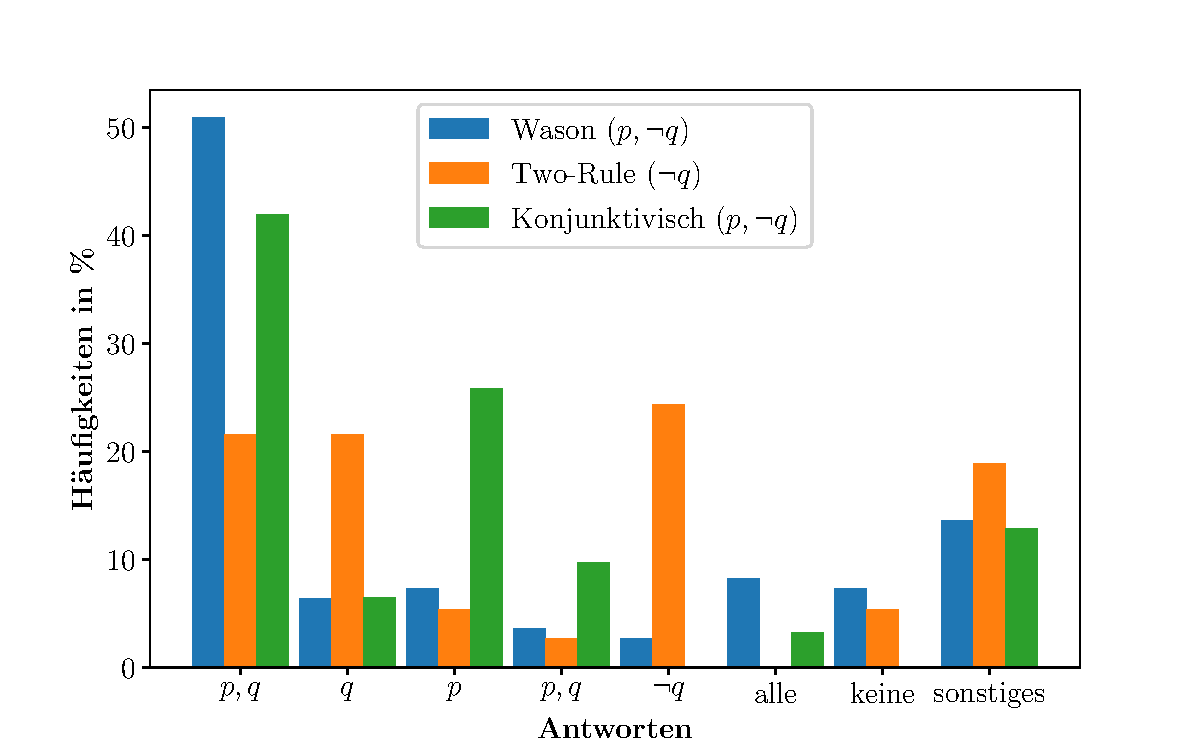
\includegraphics[width=\textwidth]{../plot/results_subjunctive.pdf}
\end{frame}


\begin{frame}{Konjunktivisch {\scriptsize \cite[S.~110]{stenningHumanReasoningCognitive2008}}}
    \begin{itemize}
        \item \emph{Every card \alert{should} have a vowel...}
        \item nicht ausreichend, um deontische Interpretation hervorzurufen
        \item alternative epistemische\footnote[frame]{\scriptsize erkenntnistheoretisch} Interpretationen von \emph{should}
        \item deontische Interpretation benötigt inhaltliche Unterstützung
        
        \item Fehlschlag der einfachsten Manipulation zum Test der These
        \begin{itemize}
            \item Interpretation als Beweis gegen Theorie?
            \item \textsc{Stenning} und \textsc{Lambalgen}: weitere Untersuchungen notwendig
        \end{itemize}
    \end{itemize}
\end{frame}


\begin{frame}{Putting it all Together {\scriptsize \cite[S.~110-112]{stenningHumanReasoningCognitive2008}}}
    \begin{itemize}
        \item Ergebnisse entsprechen Tutoren-Dialoge (Kapitel 3)
        \item Manipulationen senken Interpretationsschwierigkeiten \\
            $\Rightarrow$ Indiz für Beitrag verschiedener Problemquellen
        \item semantische Herausforderungen deskriptiver Aufgaben
        
        \item entgegen Theorien\footnote[frame]{\scriptsize außer Information-Gain (aber andere Probleme)}, die annehmen, dass
        \begin{itemize}
            \item klassische Logik die korrekte Interpretation ist und
            \item dies Interpretation der Proband:innen sei
        \end{itemize}
    \end{itemize}
\end{frame}
